\section{Methodology}\label{sec:method}

\begin{figure*}[t]
    \centering
    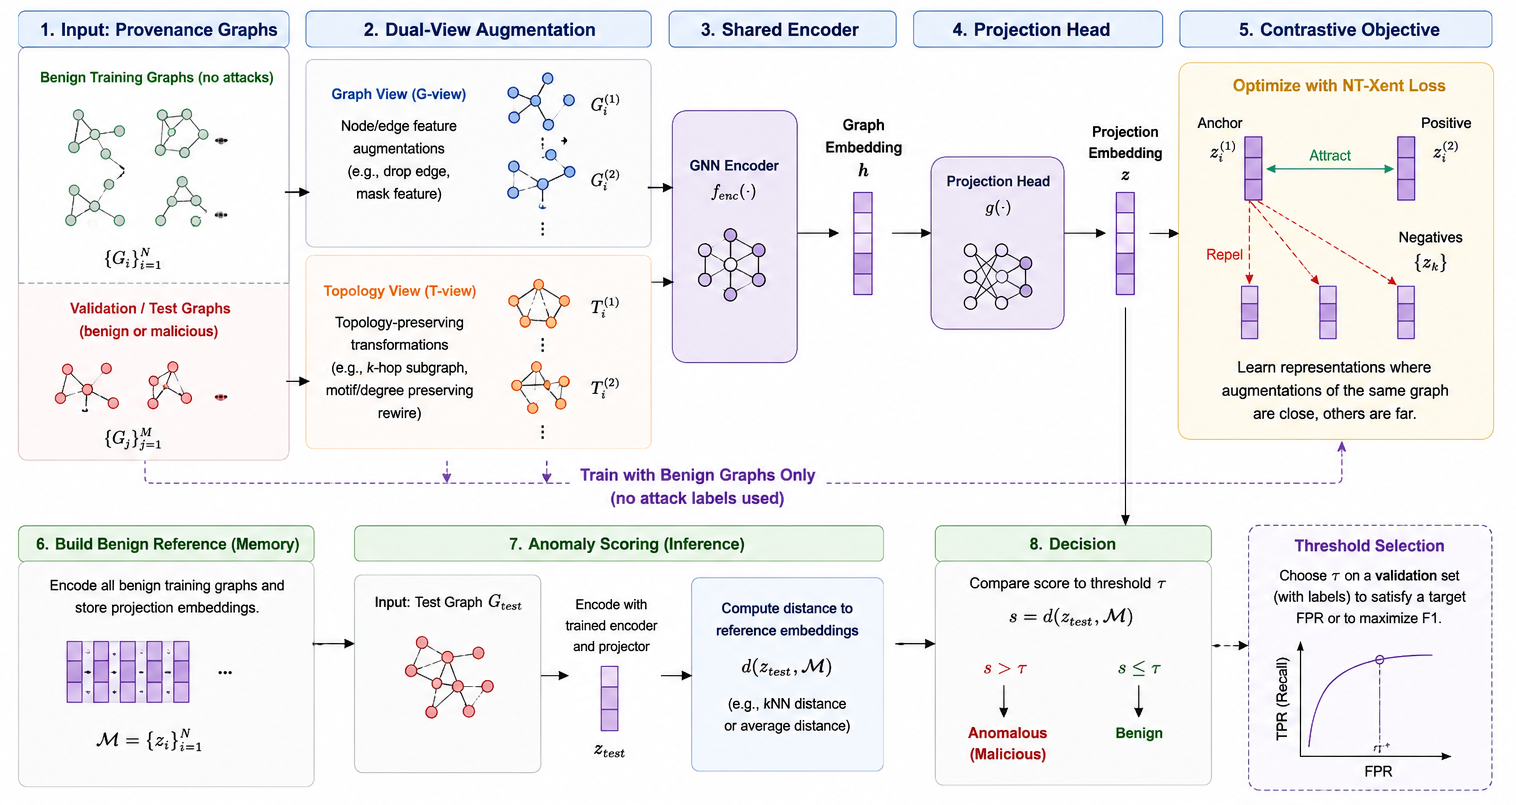
\includegraphics[width=\textwidth]{fig/method.png}
    \caption{
    Overview of \sysname{}. The top row shows contrastive training. Activity graphs are augmented into graph and topology views, encoded, projected, and optimized with a contrastive objective. The bottom row shows inference. Each graph is scored by distance to the non-malicious reference memory and classified using a validation-selected threshold.
    }
    \label{fig:method}
\end{figure*}

\sysname{} is an anomaly detection method for graph-based intrusion detection. It has four main steps. First, system activity is represented as a graph. Second, \sysname{} learns graph and topology embeddings from non-malicious training graphs using contrastive learning. Third, each validation or test graph is embedded in the same contrastive space used during training. Fourth, the detector assigns an anomaly score by measuring distance from non-malicious training embeddings. The subsections below follow this pipeline: problem setup, graph representation, contrastive training, anomaly scoring, and thresholding.

Let $G_i=(V_i,E_i,X_i)$ denote the $i$th activity graph. Here, $V_i$ is the set of nodes, $E_i$ is the set of edges, and $X_i$ is the node feature matrix. Nodes can represent entities such as hosts, devices, services, processes, or files. Edges represent interactions such as communication, access, or system events.

Let $\mathcal{B}_{\text{train}}=\{G_i : y_i=0\}$ be the training set, where $y_i=0$ means non-malicious and $y_i=1$ means malicious. During representation learning, \sysname{} uses only graphs from $\mathcal{B}_{\text{train}}$. Malicious graphs are not used to train the encoder or projection head. They are used only during validation for threshold selection and during testing for evaluation.

The goal is to learn an embedding function $f(\cdot)$ that maps each graph $G_i$ to a vector representation. At test time, graphs that are far from the non-malicious training distribution receive higher anomaly scores. This setting differs from supervised graph classification. A supervised graph neural network learns directly from both benign and malicious labels. \sysname{} instead learns normal behavior from benign graphs and detects graphs that do not match that learned normal pattern.

\subsection{Graph and Topology Representations}

\sysname{} uses two complementary views of each graph: a graph-structure view and a topology view.

The graph-structure view is learned with a graph neural network encoder. In our implementation, this encoder is a graph isomorphism network. The encoder performs message passing over the graph and pools node embeddings into one graph-level readout. We use sum, mean, and max pooling and concatenate the three pooled vectors. This produces a raw graph readout, denoted by $h_i$.

The raw readout $h_i$ is then passed through a projection head. The projection head maps $h_i$ into a contrastive graph embedding, denoted by $z_i^{G}$. This embedding is the graph-channel representation used by the contrastive loss.

The topology view captures graph shape more directly. For each graph, \sysname{} computes topological summaries from structural node scores such as degree and closeness. These summaries describe how connected components appear and merge as the graph is viewed through a filtration. The topological summaries are converted into fixed-length vectors and passed through a small multilayer perceptron. The output is a topology embedding, denoted by $z_i^{T}$.

The final contrastive embedding for graph $G_i$ combines the graph-channel and topology-channel embeddings:
\begin{equation}
    e_i =
    \left[
    \operatorname{norm}(z_i^{G})
    \; \Vert \;
    \operatorname{norm}(z_i^{T})
    \right],
    \label{eq:joint-embedding}
\end{equation}
where $\operatorname{norm}(\cdot)$ denotes $\ell_2$ normalization and $\Vert$ denotes vector concatenation. Eq.~\eqref{eq:joint-embedding} defines the embedding used later for anomaly scoring. If only one channel is used in an ablation, then $e_i$ contains only that channel.

\subsection{Contrastive Training}

During training, \sysname{} creates two augmented views of each graph. These views preserve the main identity of the graph while changing small details. For the graph channel, we use graph augmentations such as node dropping, edge dropping, and feature masking. For the topology channel, we perturb the topology feature vector with masking and noise.

InfoNCE trains the representation by posing a matching problem within each batch. For every embedding from the first augmented view, the corresponding embedding of the same original graph in the second view is the positive match; embeddings of the other graphs are alternatives. The loss increases the positive pair's similarity relative to all alternatives, with the temperature controlling how strongly it emphasizes the closest matches. Thus, the objective preserves graph identity under small augmentations while separating different benign activity patterns. Formally, for a batch of $N$ graphs, let $A=\{a_1,\ldots,a_N\}$ and $B=\{b_1,\ldots,b_N\}$ denote the embeddings of the two views. The one-direction InfoNCE loss is:
\begin{equation}
    \mathcal{L}_{\text{NCE}}(A,B)
    =
    -\frac{1}{N}
    \sum_{i=1}^{N}
    \log
    \frac{
        \exp(\operatorname{sim}(a_i,b_i)/\tau)
    }{
        \sum_{j=1}^{N}
        \exp(\operatorname{sim}(a_i,b_j)/\tau)
    },
    \label{eq:infonce}
\end{equation}
where $\operatorname{sim}(\cdot,\cdot)$ is cosine similarity and $\tau$ is a temperature parameter. Eq.~\eqref{eq:infonce} makes embeddings from two views of the same graph closer and pushes embeddings from different graphs apart. In practice, we use the symmetric version by averaging $\mathcal{L}_{\text{NCE}}(A,B)$ and $\mathcal{L}_{\text{NCE}}(B,A)$.

The full training loss combines the graph-channel contrastive loss and the topology-channel contrastive loss:
\begin{equation}
    \mathcal{L}
    =
    \alpha \mathcal{L}_{G}
    +
    \beta \mathcal{L}_{T},
    \label{eq:training-loss}
\end{equation}
where $\mathcal{L}_{G}$ is the graph-channel loss, $\mathcal{L}_{T}$ is the topology-channel loss, and $\alpha$ and $\beta$ control their weights. Eq.~\eqref{eq:training-loss} trains \sysname{} to learn both local graph structure and higher-level topology from graphs.

\subsection{Contrastive-Space Anomaly Scoring}

After training, \sysname{} embeds every training graph using the trained model. Let
$\mathcal{E}_{\text{benign}}=\{e_j : G_j \in \mathcal{B}_{\text{train}}\}$
be the set of benign training embeddings.

For a validation or test graph $G_i$, \sysname{} computes its embedding $e_i$ using Eq.~\eqref{eq:joint-embedding}. It then compares $e_i$ with the training embeddings. The anomaly score is the average distance to the $k$ nearest embeddings:
\begin{equation}
    s(G_i)
    =
    \frac{1}{k}
    \sum_{e_j \in \operatorname{kNN}(e_i,\mathcal{E}_{\text{benign}})}
    \lVert e_i-e_j\rVert_2 .
    \label{eq:knn-score}
\end{equation}
Eq.~\eqref{eq:knn-score} assigns a larger score to graphs that are farther from normal training graphs. These graphs are more likely to be anomalous.

The key design choice in \sysname{} is that anomaly scoring uses the same contrastive embedding space shaped during training. Some contrastive pipelines train a projection head but later score graphs using the raw encoder readout $h_i$. This can create a mismatch because the contrastive objective directly optimizes the projected embedding, not the raw readout. \sysname{} avoids this mismatch by scoring graphs with $e_i$, which is built from the contrastive embeddings. This keeps training and detection consistent.

\subsection{Detection and Thresholding}

The anomaly score $s(G_i)$ is converted into a binary prediction using a threshold $\gamma$:
\begin{equation}
    \hat{y}_i =
    \begin{cases}
    1, & s(G_i) \geq \gamma,\\
    0, & s(G_i) < \gamma,
    \end{cases}
    \label{eq:threshold}
\end{equation}
where $\hat{y}_i=1$ means the graph is predicted as malicious and $\hat{y}_i=0$ means it is predicted as non-malicious. Eq.~\eqref{eq:threshold} defines the final detection rule.

In our experiments, $\gamma$ is selected on the validation set. The validation set contains both non-malicious and malicious graphs so that we can choose the threshold that gives the best validation F1 score. The selected threshold is then fixed and applied once to the test set. The encoder and projection head are still trained only on benign graphs. Malicious labels are used for threshold selection and evaluation, not for representation learning.
